\chapter{Simulation study}
\label{chap:SimulationStudy}

\section{Introduction}
In order to study the methods in more depth a simulation study will be done. The main advantage of this simulation study over using data on real species is that the variables that make up the species distribution can be decided upon. Because of the usual non-linear shape of the response-functions, the sampling design, \dots it is quite hard to set up a simulation study. Luckily the
\textsc{virtualspecies} package \parencite{virtualspecies, leroy2015virtualspecies} provides a simulation framework that allows the simulation of realistic species distributions. \\

\section{Overview of the \textsc{virtualspecies} package and the simulation set-up}
In order to justify using the samples generated by the \textsc{virtualspecies} package the internal process is quickly sketched. \\

First of all, the \textsc{virtualspecies} package generates a suitability raster, i.e.\ a raster containing high values for suitable habitat and vice versa, based upon a set of provided rasters of environmental variables. Since the package imposes no restrictions on the function that generates the suitability from the provided variables, the suitability raster has to be converted into a probability of occurrence map. This can be done by using e.g.\ the logit function to map $\mathbb{R} \to [0,1]$. Once a raster containing the occurrence probability map is obtained a raster containing ones where the simulated species is present and zeroes otherwise can be obtained. This is done by sampling cells with a probability proportional to the probability of the occurrence and setting the cell value to $1$. Trom this raster a presence-only sample can be obtained by drawing random points within the cells that have a value of $1$.\\

To facilitate the computations it was decided to select one area in which several random species are generated. In order to make sure that the environmental conditions can fluctuate within the distribution of one generated species to the next it was required that the selected area has to contain different types of habitat types. The obvious choice would be to use the contiguous United States, this is, however, computationally demanding. In the end it was decided to perform the simulation study on data contained within a rectangle that approximately corresponds to Washington state, see Figure \ref{fig:WashState}. Washington state has a big precipitation and temperature gradient because of the rain shadow created by the Cascade Range. This is also reflected in the fact that the types of habitat within this extent range from temperate rainforests, e.g.\ the Hoh Rainforest, to steppe- and dessert-like areas in Southeastern Washington. \\

\begin{figure}[!htb]
\center
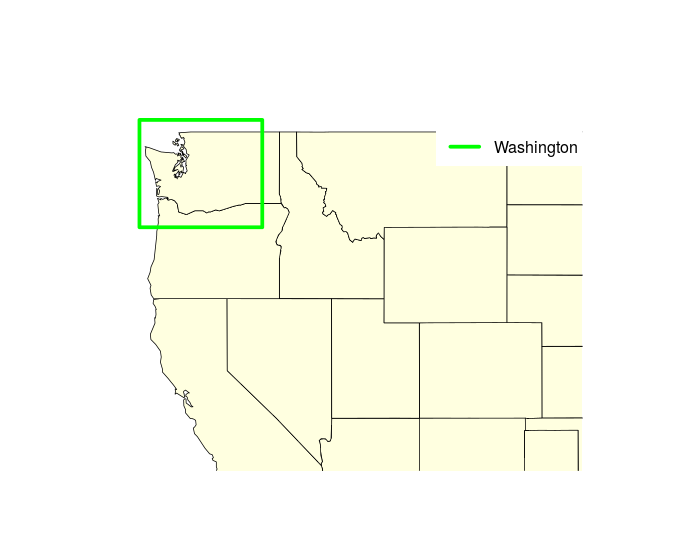
\includegraphics[scale=0.5]{Plots/WashingtonPlot.png}
\caption{\label{fig:WashState}Extent considered in the simulation study.}
\end{figure}

In order to study the generalizability of the methods it was decided that $5$ different species would be simulated. Furthermore, to be able to investigate the sample to sample variability of each method $5$ different presence-only samples were drawn for each simulated species. Since the mean (resp.\ median) number of observations of the presence-only datasets is $320.3$ (resp.\ $133.5$) it was decided to simulate $200$ occurrence points for each simulated dataset. \\

In Section \ref{sec:AUC} the various sources of the variability in the AUC values were discussed. Given that the interest is mainly in the training sample to training sample variability, it was decided to try to restrict the test sample to test sample variability to some extent. This can be done by taking a large test set. Using a sample of $1000$ occurrence and $1000$ background locations the standard error of the AUC value, conditional on the classifier, is $\approx 0.013$. This should be large enough to prevent the scenario where the test sample to test sample variability is much larger than the training to training sample variability.

\section{Model}

In order to be able to perform statistical inference an underlying model has to be proposed and estimators will be proposed. First of all the generated AUC values will be denoted by $Y_{ij}$ with $i \in \{1,\ldots,5\}$ indicating the species and $j \in \{1,\ldots,5\}$ indicates which sample of the $i$'th virtual species is considered. We assume that there is an underlying average AUC value $\mu$, for each sampled species there is then a species specific average AUC that deviates from $\mu$ by an amount equal to $\delta_i$ with $E(\delta_i) = 0$. Finally, because of training and test sample variability the estimated AUC will deviate from $\mu + \delta_i$ by an error $\epsilon_{ij}$ with $E(\epsilon_{ij} = 0$. Hence:
\[Y_{ij} = \mu + \delta_i + \epsilon_{ij}.\]
It is logically to assume that not only the $\delta_i$ and $\epsilon_{ij}$ are random but also that the $Var(\epsilon_ij) = \sigma_i^2$ is a species specific variance that is different for each species. For each method we are interested is in estimating:
\begin{itemize}
\item The mean $\mu$.
\item The species to species variance or thus $V(\delta)$
\item The expected variation of a classifier ``independent'' of the selected species or hence $E(\sigma^2)$.
\item The difference between using all variables or only the bioclimatic variables, i.e. $\mu_{all} - \mu_{bio}$.
\end{itemize} 

First of all the usual unbiased estimator of $\sigma_i^2$ is $\sum_{j= 1}^{5} \frac{Y_{ij} - \bar{Y}_i}{4} $, with $\bar{Y}_i = \frac{\sum_{j=1}{5}Y_{ij}}{5}$.
In order to estimate $E(\tau)$ we note that 
\[E\left(\frac{1}{5} \sum_{j= 1}^{5} \frac{Y_{ij} - \bar{Y}_i}{4}\right) = E\left\lbrace \frac{1}{5} \sum_{i=1}^5 E\left( \sum_{j= 1}^{5} \frac{Y_{ij} - \bar{Y}_i}{4}  \bigg\vert \sigma_1^2, \ldots, \sigma_5^2 \right) \right\rbrace = \frac{1}{5} \sum_{i=1}^5 E \left( \sigma_i ^ 2 \right) = E\left( \sigma^2 \right). \]

Furthermore
\[E\left(\sum_{i=1}^5 \sum_{j=1}^5 \frac{Y_{ij}}{25} \right) = \sum_{i=1}^5 \sum_{j=1}^5 \frac{E(Y_{ij})}{25} = \sum_{i=1}^5 \sum_{j=1}^5 \frac{\mu}{25}.\]

\section{Results}



\begin{figure}[!htb]
\center
\makebox[\textwidth][c]{%
	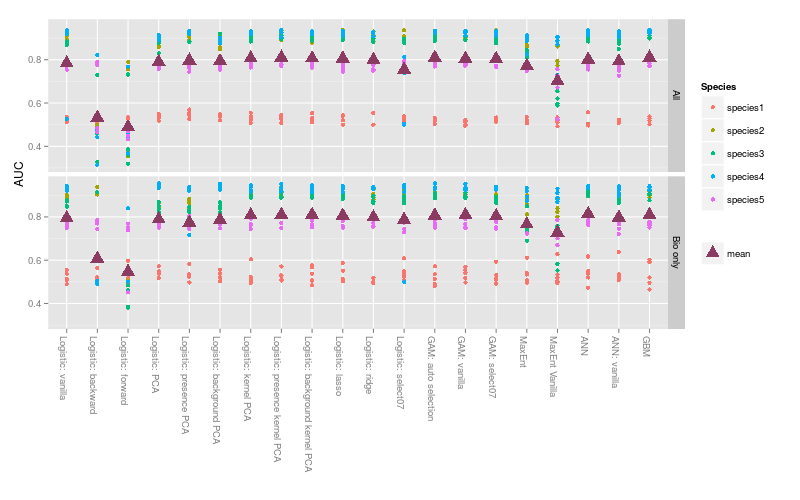
\includegraphics[scale=0.70]{Plots/SimulationAUC.png}
}
\caption{\label{fig:PrAbAUC}AUC values of the different classifiers fitted on the simulated data.}
\end{figure}


\begin{figure}[!htb]
\center
\makebox[\textwidth][c]{%
	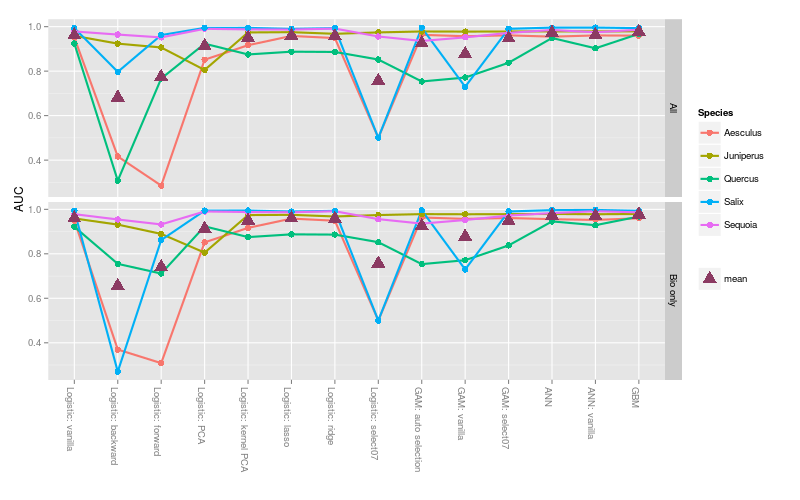
\includegraphics[scale=0.70]{Plots/AUCPAPlot.png}
}
\caption{\label{fig:PrAbAUC}Difference between the AUC values when using all versus only the bioclimatic variables.}
\end{figure}

\section{Discussion}





